\documentclass{article}
\usepackage[utf8]{inputenc}
\usepackage{authblk}
\usepackage{setspace}
\usepackage[margin=1.25in]{geometry}
\usepackage{graphicx}
\graphicspath{ {./figures/} }
\usepackage{amsmath,amssymb,amsfonts}
\usepackage{booktabs}
\usepackage{natbib}
\usepackage{hyperref}
\hypersetup{colorlinks=true, linkcolor=blue, citecolor=blue, urlcolor=blue}

\title{\textbf{Gradient-Boosted Ranking of Next-Week Returns in US Mega-Cap Equities: A Walk-Forward Test}}
\author[1]{hypoq autonomous research harness}
\affil[1]{Hypothesis $\times$ Quant}
\date{\today}
\onehalfspacing

\begin{document}
\maketitle

\begin{abstract}
\noindent \textbf{Hypothesis:} $H_0$: the out-of-sample mean cross-sectional rank IC of a gradient-boosting forecast of the 5-day return is zero; $H_1$: it is positive \\
\textbf{Data:} Daily prices and volume of 35 US mega-cap stocks, out-of-sample 2019-01-02 to 2026-10-16 (1,959 days) \\
\textbf{Method:} Walk-forward from 2019 with annual retraining, a 10-day embargo, cross-sectionally rank-normalised features, ridge and 12-1 momentum benchmarks, HAC (5 lags) inference \\
\textbf{Results:} GBM mean IC 0.0133 (HAC $t=1.80$, one-sided $p=0.036$); ridge -0.0048; momentum 0.0106. Decision: \textbf{ACCEPTED}
\end{abstract}

\section{Design}
Features are 1/5/21/63-day returns, 12-1 momentum, 21/63-day volatility, their ratio and a volume z-score, each rank-normalised across stocks on the same date. The label is the cross-sectional rank of the close-to-close return from $t$ to $t+5$. Models are refit each January on data that end ten calendar days earlier, so no label overlaps the test year \citep{gu2020empirical}.

\section{Results}
\begin{table}[H]
\centering
\caption{Out-of-sample daily rank IC against the 5-day forward return}
\begin{tabular}{lcccc}
\toprule
Model & Mean IC & HAC $t$ & One-sided $p$ & Days IC $>0$ \\
\midrule
gbm & 0.0133 & 1.80 & 0.0363 & 52.7\% \\
ridge & -0.0048 & -0.43 & 0.6650 & 50.3\% \\
momentum & 0.0106 & 0.86 & 0.1957 & 51.8\% \\
\bottomrule
\end{tabular}
\end{table}


Gross of costs, the top-third minus bottom-third GBM spread earns 0.120\% per 5 days (HAC $t=1.56$).

\begin{figure}[h!]
\centering
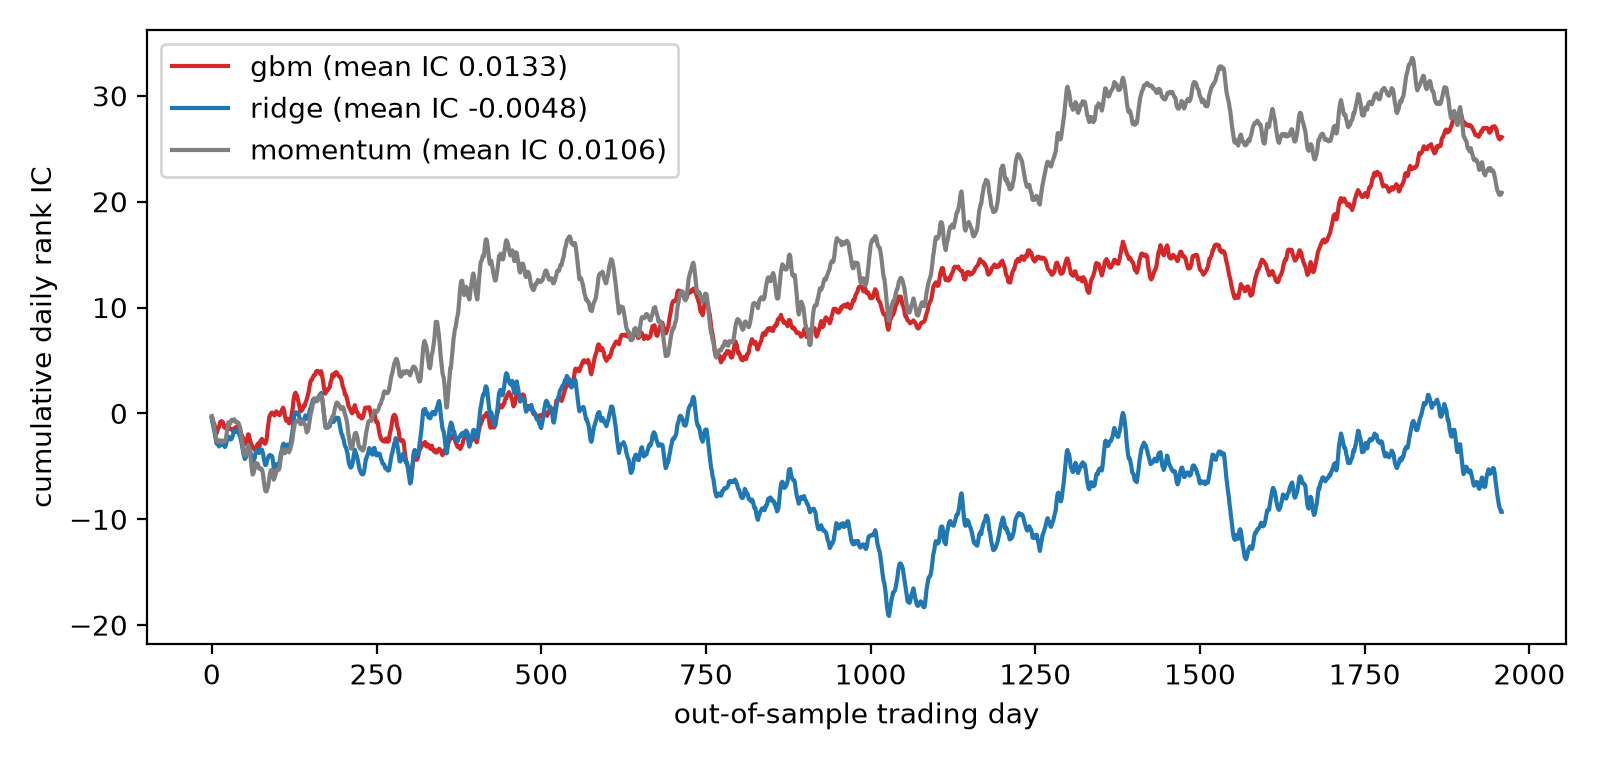
\includegraphics[width=0.85\textwidth]{fig1_cumulative_ic.png}
\caption{Cumulative daily rank IC.}
\end{figure}

\section{Limitations}
The universe consists of today's mega-caps, which is survivorship-biased and flatters every model; with only 35 names the daily IC is noisy; spreads ignore trading costs and borrow fees.


\bibliographystyle{plainnat}
\bibliography{references}

\end{document}
